
\documentclass[journal,twoside]{IEEEtran}
%\documentclass[draftcls]{IEEEtran}


%\usepackage[english]{babel} 
\usepackage{soul}

\usepackage{cite}

\usepackage[pdftex]{graphicx}
\graphicspath{{img/}}

\usepackage[cmex10]{amsmath}
\usepackage{amssymb}
\interdisplaylinepenalty=2500
\usepackage{array}
\usepackage{mdwmath}
\usepackage{mdwtab}
\usepackage{eqparbox}
\hyphenation{op-ti-cal net-works se-mi-con-duc-tor har-mo-nics har-mo-nic}
\renewcommand{\vec}[1]{\mathbf{#1}}
\newcommand{\mat}[1]{\mathbf{#1}}
\usepackage{color}


\begin{document}

%\nocite{*}

\title{Efficient Harmonic Balance Analysis of \\ Waveguide Devices with Nonlinear Dielectrics}
\author{ Laurent~Ntibarikure,~\IEEEmembership{Student 
        Member,~IEEE,}
		Giuseppe~Pelosi,~\IEEEmembership{Fellow,~IEEE,}
        and~Stefano~Selleri,~\IEEEmembership{Senior~Member,~IEEE}
        \thanks{ L. Ntibarikure, G. Pelosi and S. Selleri are with the
        Department of Electronics and Telecommunications, University of 
        Florence, Via di S. Marta, 3, I-50139 Florence, Italy (e-mail:
        laurent.ntibarikure@unifi.it; giuseppe.pelosi@unifi.it; stefano.selleri@unifi.it). }}

\markboth{IEEE MICROWAVE AND WIRELESS COMPONENTS LETTERS, VOL. X, NO. X, Month XXXX}
{IEEE MICROWAVE AND WIRELESS COMPONENTS LETTERS, VOL. X, NO. X, Month XXXX}

\maketitle

\begin{abstract}
The computation of high order harmonic components of the time-harmonic field
originated in waveguide structures containing nonlinear dielectrics is addressed
exploiting harmonic balance and finite element methods. The solution of the
nonlinear system is handled either via Picard or relaxed iterations. Being the
nonlinear loop particularly time demanding, a domain decomposition method is 
proposed to speed-up the system solution by restricting the iteration to a small
subdomain. A numerical example over a \mbox{2-D} H-plane device is presented.
\end{abstract}

\begin{IEEEkeywords}
Harmonic analysis, finite element methods, domain decomposition method,
nonlinear media, waveguide filters.
\end{IEEEkeywords}

\IEEEpeerreviewmaketitle

\section{Introduction}

\IEEEPARstart{T}{ime-domain} analysis of waveguide devices including nonlinear
dielectrics often results to be computationally prohibitive \cite{deGersem2001}.
A time-harmonic finite element (FE) approach at a single frequency is not 
sufficient to include all relevant phenomena. 
Higher order harmonics are needed and may be taken into account by using the 
harmonic balance finite element (HBFE) method \cite{Yamada1989}, also known as 
multiharmonic finite element method \cite{Copeland2010}, which provides a fast 
and accurate solution for low frequency problems.
In this framework, an algebraic domain decomposition (DD) technique was
proposed to improve computational timings also in high frequency
problems \cite{Guarnieri2010}, but no harmonic balance
was present there and hence only the fundamental frequency was evaluated.
In this letter, \cite{Guarnieri2010} is expanded by implementing a full
harmonic balance domain decomposition finite element (HBDDFE) method for
solving Helmholtz equation. The capability and efficiency of the method are
proved on an H-plane waveguide filter example.

%%%%%%%%%%%%%%%%%%%%%%%%%%%%%%%%%%%%%%%%%%%%%%%%%%%%%%%%%%%%%%%%%%%%%%%%%%%%%%%%
\section{Formulation}
\label{sec:Formulation}
%
% \begin{figure}[t!]
% \centering
% 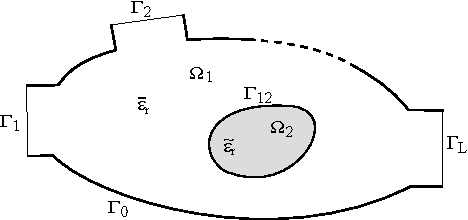
\includegraphics{geometryLarge}
% \caption{Generic multiport device where the total domain $\Omega$ is subdivided
% into a large, linear subdomain $\Omega_1$ and a smaller subdomain $\Omega_2$.}
% \label{fig:geometry}
% \end{figure}
%The HBFE formulation is presented here for the special case of an H-plane 
%waveguide filter, a, but the extension to the \mbox{3-D} case is straighforward
%
Given a generic multiport device, 
% Given the microwave device of Fig.~\ref{fig:bilat}, 
its domain $\Omega$ either in \mbox{2-D} or \mbox{3-D} Euclidean space
%, with boundary $\Gamma$,
can be divided into a large part $\Omega_1$ comprising only linear media, and 
a small part $\Omega_2$ comprising all nonlinear media.
%\st{, with $\Omega = \Omega_1 \cup \Omega_2$ and
%$\Omega_1 \cap \Omega_2 = \emptyset$}
Permittivity in $\Omega$ can be expressed as
\begin{equation}
\varepsilon_r(\vec{E}(\vec{r}),\vec{r})\!=\! 
\begin{cases}
\bar{\varepsilon}_r(\vec{r}), & \vec{r} \in \Omega_1 \\
\tilde{\varepsilon}_r(\vec{E}(\vec{r}), \vec{r}) \!=\!
\bar{\varepsilon}_r(\vec{r}) \!+\! \mathcal{L}(\vec{E}(\vec{r})), & \vec{r} \in
\Omega_2
\end{cases}
\end{equation} 
%
\noindent where $\vec{E}(\vec{r})$ is the electric field in the generic point
$\vec{r}$ and $\mathcal{L}(\cdot)$ denotes a generic scalar operator describing 
the nonlinear behavior \cite{Guarnieri2010}. The electric field satisfies, 
within $\Omega$, the well known vector Helmholtz equation 
%\cite{Pelosi2009}
%
%\begin{equation}
%\label{eq:helmholtz}
%\nabla \times \left ( \frac{1}{\mu_r} \nabla \times \vec{E}(\vec{r}) \right ) 
%- {k}^2 \varepsilon_r \left(\vec{E}(\vec{r}), \vec{r} \right) \vec{E}(\vec{r})
%= 0
%\end{equation} 
with suitable boundary conditions on $\Gamma$. For the example shown 
in Section~\ref{sec:results} (Fig.~\ref{fig:bilat}), $\Gamma$
comprises a part $\Gamma_0$ which will be considered perfect electric conductor,
and two parts $\Gamma_1$ and $\Gamma_2$ 
%$L$ parts $\Gamma_l$
corresponding to the ports where a modal expansion is enforced \cite{Pelosi2009}. 
$\Gamma_{12}$ corresponds to the internal boundary between subdomains $\Omega_1$
and $\Omega_2$.

In a standard FE Galerkin framework the domain $\Omega$ is
discretized into a set of non overlapping finite elements and the electric
field is approximated, in the \mbox{3-D} case, as a linear combination of vector (edge) 
basis functions $\boldsymbol{\alpha}_n$. In the H-plane (\mbox{2-D}) case treated in
Section~\ref{sec:results}, 
%the vector basis functions are written as 
scalar nodal basis functions multiplyed by the out-of-plane unit vector (TM problem) are employed.
%
%\begin{equation}\label{e:femexpansion}
%\vec{E}(\vec{r})  = \sum_{n=1}^N E_n \boldsymbol{\alpha}_n(\vec{r})
%\end{equation} 
%
By testing 
%\eqref{eq:helmholtz} 
Helmholtz equation over $\Omega$ with weighting functions
$\boldsymbol{\alpha}_m$, chosen equal to the basis, the following weak form is
obtained:
%
\begin{multline}\label{eq:fem}
\hspace{-.4cm}\int_\Omega \nabla \times \boldsymbol{\alpha}_m (\vec{r}) \cdot \frac{1}{\mu_r}
\nabla \times \vec{E}(\vec{r}) \ d\Omega 
- k^2 \int_\Omega \boldsymbol{\alpha}_m (\vec{r}) \cdot \varepsilon_r 
(\vec{E}(\vec{r}), \vec{r})  \\ 
  \vec{E}(\vec{r}) \ d\Omega
+ \oint_{\Gamma} \boldsymbol{\alpha}_m (\vec{r}) \cdot \hat{n} \times 
\frac{1}{\mu_r} 
\nabla \times \vec{E}(\vec{r}) \ d\Gamma = 0
\end{multline} 
%
\noindent being $k$ the free space wavenumber. 

The multiharmonic dependence in the HBFE method is introduced
by approximating the electric field as truncated Fourier series
\cite{Copeland2010}
%
\begin{equation} \label{eq:field}
\vec{\hat{E}}(\vec{r}, t) = \sum^P_{p=1} \left( \vec{E}_{p}^{(s)}(\vec{r}) 
\sin(p\omega_0 t) + \vec{E}_p^{(c)}(\vec{r}) \cos(p \omega_0 t) \right)
\end{equation}
%
\noindent where $\omega_0$ is the fundamental angular frequency and
%\st{, here and in the following,} 
%the hat over a quantity denotes its approximated value given by
%the truncated Fourier series. 
$\vec{E}_{p}^{(s)}$ and $\vec{E}_{p}^{(c)}$ are the harmonic complex amplitudes 
that expand the field at $p\omega_0$ and hence they must individually
satisfy Helmholtz equation with $k=pk_0$. 
This is done 
%in the FE framework 
by using the FE expansion for each coefficient 
$\vec{E}_{p}^{(s)}$ and $\vec{E}_{p}^{(c)}$.
The scalar relative permittivity can also be approximated as \cite{Copeland2010}
%
\begin{eqnarray} \label{eq:eps}
\hat{{\varepsilon}}_r(\vec{E}(\vec{r}), \vec{r}, t) = {\varepsilon}_{r_0} + 
\sum^G_{g=1} \left( {\varepsilon}_{r_g}^{(s)} \sin(g \omega t) + 
{\varepsilon}_{r_g}^{(c)} \cos(g \omega t)
\right)
\end{eqnarray} 
\noindent where the coefficients of the expansion are given by
\begin{align} \label{eq:epsCoeffs}
{\varepsilon}_{r_{0}} &=  \frac{\omega}{2\pi}\int_0^{\frac{2\pi}{\omega}}
{\varepsilon}_r(\vec{E}(\vec{r}), \vec{r}) \ dt \nonumber \\
{\varepsilon}_{r_{g}}^{(s)} &=  \frac{\omega}{\pi}\int_0^{\frac{2\pi}{\omega}}
{\varepsilon}_r(\vec{E}(\vec{r}), \vec{r}) \sin(g \omega t) \ dt \\ 
{\varepsilon}_{r_{g}}^{(c)} &=  \frac{\omega}{\pi}\int_0^{\frac{2\pi}{\omega}} 
{\varepsilon}_r(\vec{E}(\vec{r}), \vec{r}) \cos(g \omega t) \ dt
\nonumber 
\end{align} 

%The orders of the approximations $P$ and $G$ reflects on the accuracy
%of the solution and can be set
%automatically in the algorithm \cite{Gyselinck2002}.
%
A conventional, linear, FE approach discretization of \eqref{eq:fem} 
%via \eqref{e:femexpansion}
leads to a system in the form [$a_{mn}][E_n] = [b_m]$ \cite{Pelosi2009}.
% %
% \begin{equation}\label{e:plainfem}
% \begin{bmatrix}
% a_{11} & a_{12} & \ldots & a_{1N} \\
% a_{21} & a_{22} & \ldots & a_{2N} \\
% \vdots & \vdots & \ddots & \vdots \\
% a_{N1} & a_{N2} & \ldots & a_{NN} \\
% \end{bmatrix}
% \begin{bmatrix}
% E_1\\
% E_2\\
% \vdots\\
% E_N
% \end{bmatrix}
% =
% \begin{bmatrix}
% b_1\\
% b_2\\
% \vdots\\
% b_N
% \end{bmatrix}
% \end{equation}
In an HBFE approach, $\vec{E}(\vec{r})$ and
${\varepsilon}_r(\vec{r})$ must be substituted by their respective harmonic 
approximations $\vec{\hat{E}}(\vec{r}, t)$ and $\hat{{\varepsilon}}_r(\vec{r}, t)$ in \eqref{eq:fem}.  By performing
a further testing with weights $\sin(q \omega t)$ or
$\cos(q \omega t)$, $q = 1 \dots P$, and integrating over the time period of the fundamental $\left [
0,\frac{2\pi}{\omega} \right ]$,  a large linear system is
obtained which has formally the same structure as 
%\eqref{e:plainfem} 
a conventional FE system but in which each entry $a_{mn}, E_n$ or $b_m$
is itself a matrix or a vector:
%
\begin{equation}\label{e:HBfemmn}
a_{mn}=
\begin{bmatrix}
a_{mn}^{(1s1s)} & a_{mn}^{(1s1c)} & \ldots &  a_{mn}^{(1sPc)} \\
a_{mn}^{(1c1s)} & a_{mn}^{(1c1c)} & \ldots &  a_{mn}^{(1cPc)} \\
\vdots & \vdots & \ddots & \vdots \\
a_{mn}^{(Pc1s)} & a_{mn}^{(Pc1c)} & \ldots &  a_{mn}^{(PcPc)}
\end{bmatrix}
\end{equation}
\begin{equation} 
E_n = 
\begin{bmatrix}
E_{n}^{(1s)} &
E_{n}^{(1c)} &
\ldots &
E_{n}^{(Pc)}
\end{bmatrix}^\text{T}
\end{equation}
\begin{equation}
b_m = 
\begin{bmatrix}
b_{m}^{(1s)} &
b_{m}^{(1c)} &
\ldots &
b_{m}^{(Pc)}
\end{bmatrix}^\text{T}
\end{equation}

\noindent The superscripts $(q[s|c])$ and $(p[s|c])$ indicates that the corresponding
entry was computed by testing \eqref{eq:fem} with $[\sin(q \omega t) | \cos(q \omega t)]$ 
while the corresponding harmonic basis in \eqref{eq:field}
was $[\sin(p \omega t) | \cos(p \omega t)]$.

The nonlinearity is finally handled via a
relaxed iteration. As a starting point a null electric field $[E]^0$ is assumed,
computing the pertinent system matrix $[A_{([E]^0)}]$ and
known term $[b_{([E]^0)}]$ and solving the system $[A_{([E]^0)}] [E]^1 =
[b_{([E]^0)}]$. The newly computed field $[E]^1$ can now be used to update system
matrix and known term and perform the following relaxed iteration:
% %
\begin{equation} \label{eq:lastLinearSystem}
 [A_{(\gamma [E]^{i-1} + (1-\gamma) [E]^{i-2})}] [E]^{i} = [b_{(\gamma [E]^{i-1}
 + (1-\gamma) [E]^{i-2})}]
\end{equation}
% \begin{equation} \label{eq:lastLinearSystem}
% [A]^{i-1} [E]^{i} = [b]^{i-1}
% \end{equation}
% 
% \noindent with 
% %
% \begin{align}
% [A]^{i-1} &= [A_{(\gamma [E]^{i-1} + (1-\gamma) [E]^{i-2})}] \\
% [b]^{i-1} &= [b_{(\gamma [E]^{i-1} + (1-\gamma) [E]^{i-2})}]
% \end{align}

\noindent with $i \geq 2$ and
$\gamma\in(0,1]$. $\gamma=1$ gives the standard Picard iteration 
\cite{Guarnieri2010}, while low $\gamma$ values damps the oscillations
which may arise with highly nonlinear materials or high intensity impressed
fields at the cost of a slower convergence \cite{Silvester1997}. The process 
is repeated until the relative error between the updated solution
and the previous one, in the sense of the Euclidean norm, is less than a
prescribed value $\tau$ \cite{Guarnieri2010}.

The order of the resulting HBFE system is $2 N P$, and
this number can become very high, and, since the
solutions have to be refined iteratively building at each step a new linearized
system, computing time can become too high.
To enhance the computational efficiency, a substructuring DD
approach is here proposed \cite{Guarnieri2010,Guarnieri2009}. The multiharmonic
unknowns vector $[E]$ defined by the HBFE method over $\Omega$ can be split
into two vectors $[E^{(1)}]$ and $[E^{(2)}]$ containing the unknowns belonging
to interior points in $\Omega_1$ and $\Omega_2$, respectively. Unknowns
belonging to the boundaries $\Gamma\cup\Gamma_{12}$ are placed in a third
vector $[E^{(c)}]$. The HBFE system can then be recast in:
%
\begin{equation}\label{eq:DD}
\begin{bmatrix}
 [M^{(1)}] &  \!\!0\!\!  &  [P^{(1)}] \\
 0  &  \!\![M^{(2)}]^{i-1}\!\! & [P^{(2)}]^{i-1} \\
 [Q^{(1)}] & \!\![Q^{(2)}]^{i-1}\!\! & [C]^{i-1}
\end{bmatrix}
\!\!\!\!
\begin{bmatrix}
{[E^{(1)}]^{i}} \\
{[E^{(2)}]^{i}} \\
{[E^{(c)}]^{i}}
\end{bmatrix} 
\!\!\!=\!\!\!
\begin{bmatrix}
{[b^{(1)}]} \\
{[b^{(2)}]}^{i-1} \\
{[b^{(c)}]}^{i-1}
\end{bmatrix} 
\end{equation}

\noindent where $[M^{(1)}]$ contains the HBFE coefficients of the linear system
related to the unknowns $[E^{(1)}]$, with
null harmonic coupling coefficients, while $[M^{(2)}]$ contains coefficients for
the nonlinear subdomain $\Omega_2$. ${[P^{(\cdot)}]}$ and ${[Q^{(\cdot)}]}$
represent couplings between interior unknowns and 
boundary unknowns collected in $[E^{(c)}]$. 
By using the Schur complement concept, the boundary unknowns $[E^{(c)}]^{i}$ of
\eqref{eq:DD} and hence the generalized scattering matrix of the device can be 
retrieved with the same accuracy of the full domain solution \cite{Guarnieri2009}.
Thus, in order to solve the HBDDFE system, 
every single submatrix is assembled at first sight, then, within the iteration
loop, only the submatrices related to $\Omega_2$ and $\Gamma_{12}$ are to be
updated. The efficiency of this DD technique relies on the restriction of matrices
updates to sufficiently small regions along the nonlinear iterative solution, 
noticeably improving long nonlinear loops.

%%%%%%%%%%%%%%%%%%%%%%%%%%%%%%%%%%%%%%%%%%%%%%%%%%%%%%%%%%%%%%%%%%%%%%%%%%%%%%%%
\section{Numerical Results}
\label{sec:results}

\begin{figure}[t!]
\centering

\includegraphics{bilat}
\caption{H-plane cross section of a D-Band passband filter (dielectric slab is
shown in light grey; metalization is shown as thick black lines) in a WR6 
waveguide. Measures are given in $\mu{m}$.}
\label{fig:bilat}
\end{figure}

A millimeter wave passband filter in WR6 (1651x825.5~$\mu$m) rectangular 
waveguide is here analyzed \cite{Guarnieri2010}.
%, Bui1984}. 
The filter, uniform along $y$ axis, is realized by placing on the E-plane a 
dielectric slab partially 
metalized on both sides as shown by the H-plane cross
section of Fig.~\ref{fig:bilat}. All conductors are considered perfect.
The dielectric, enclosed in $\Omega_2$, presents a Kerr-type nonlinearity of
such that \cite{Guarnieri2010}
%, Ma1997}
\begin{equation}
\tilde{\varepsilon}_r(\vec{E}(\vec{r}), \vec{r}) = \bar{\varepsilon}_r(\vec{r}) + 
\alpha_2 \ |\vec{E}(\vec{r})|^2, \qquad \vec{r} \in \Omega_2
\end{equation}
\noindent where $\bar{\varepsilon}_r(\vec{r}) = 2.1$ and 
$\alpha_2~=~1.625~10^{-10}~{\mathrm{m}^2}/{\mathrm{V}^2}$.
%is chosen as \cite{Ma1997}. 
The Kerr-like behavior
of the permittivity induces the generation of odd order harmonics, thus 
even ones can been neglected. For the relaxed
iteration stop criterion, $\tau = 10^{-6}$ has been chosen.
The continuity of the field at the ports is imposed through a modal expansion 
exploiting only $\mathrm{TE}_{m0}$ modes, $m = 2n+1$, $n=1,\ldots,4$, even $m$
modes being absent for the E-plane symmetry of the filter.  
The excitation is a $\mathrm{TE}_{10}$ mode at fundamental frequency impinging at
Port 1 with maximum field amplitude $E_ i$. The 
waveguide discontinuity represented by the filter transfers power to higher order
modes, which may result to be guided at higher harmonic frequencies.
Furthermore, as a sinusoidal excitation is chosen, only $\sin(p \omega t)$ 
related coefficients are retained.
Due to H-plane uniformity, the problem can be treated as \mbox{2-D} \cite{Pelosi2009}.
First order nodal elements are used and the discretization leads to 2473
degrees of freedom, 80 of which belong to the nonlinear subdomain $\Omega_2$, 
314 to the boundaries and 2079 to the linear subdomain $\Omega_1$. Such a fine
discretization is necessary to obtain a good approximation of the field up to 
the $5^\mathrm{th}$ harmonic.
%
\begin{figure}[!t]
\centering

\includegraphics{spectrumNHarm}
\caption{$\mathrm{TE}_{10}$ spectral response for linear (top) and nonlinear 
(bottom) permittivity with $E_i = 10$~kV/m. The results are compared with Comsol
RF module linear and nonlinear solutions.}
\label{fig:spectrumNHarm}
\end{figure}

As a first analysis, the effect of the total number of harmonics $P$
retained on the filter's spectral response is investigated
(Fig.~\ref{fig:spectrumNHarm}).  For an incident field amplitude $E_i = 10$~kV/m,
the Picard iteration proved to converge. Equal mesh and parameters have been used 
to conduct a \mbox{2-D} FE (single harmonic) analysis with Comsol RF Module 
\cite{ComsolRF}. Being the nonlinear loop tackled differently (Comsol uses Newton 
algorithm), perfect matching in the spectral response is not obtained as for the
linear permittivity case ($\alpha_2 = 0$).
%It is evident from Fig.~\ref{fig:spectrumNHarm} that including 
%the $3^\mathrm{rd}$ harmonic is crucial for proper evaluation of the device
%bandwidth. 

%\begin{figure}[!t]
%\centering
%
\includegraphics{Fields}
%\caption{$|\mathrm{E}_y|$ distribution within the filter at fundamental 
%($f_0 =$ 146 ~GHz), $3^\mathrm{rd}$ and $5^\mathrm{th}$ order harmonics 
%($\mathrm{E_i = 10 ~kV/m}$).}
%\label{fig:Fields}
%\end{figure}

\begin{figure}[!t]
\centering
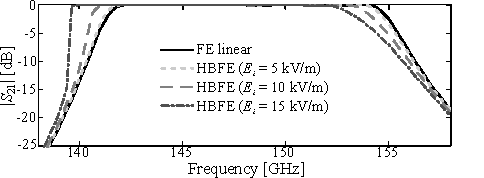
\includegraphics{spectrumS21b}
\caption{$|S_{21}|$ of the nonlinear filter for
several values of $E_i$ compared to the linear case. Field is approximated
up to the $5^\mathrm{th}$ harmonic.}
\label{fig:spectrum}
\end{figure}

To gain better insight, simulations have
been repeated with $E_i=5$~kV/m and $E_i=15$~kV/m, for $P=5$. 
The results compared to those of a linear device are shown in Fig.~\ref{fig:spectrum}. 
There is an evident shift of the band 
towards lower frequencies as higher power densities are involved, which agrees 
to \cite{Yatsyk2006}. Furthermore the $E_i=15$~kV/m did not 
converge with Picard iteration and required a relaxed $\gamma = 0.1$ iteration.
% In this case, the abrupt variation of $|S_{21}|$ around $139.5$~GHz points out 
% that $P=5$ is not sufficient to accurately analyze the device.
% Indeed, the power associated to harmonics grows as the incident field 
% increases as shown in Fig.~\ref{fig:harmSpectrum}. 
% \st{but a finer mesh would be necessary to allow for higher $P$ values.}
% \begin{figure}[!t]
% \centering
% 
\includegraphics{harmSpectrum}
% \caption{Spectral responses at $3^\mathrm{rd}$ (top) and $5^\mathrm{th}$ 
% (bottom) harmonics
% for scattered modes (Incident $\mathrm{TE}_{10}$ with (a) $E_i = 10$~kV/m;
% (b) $E_i = 15$~kV/m.}
% \label{fig:harmSpectrum}
% \end{figure}

Analysis of the spectral response convergence is performed computing the relative
error, in Euclidean norm sense, all over the device bandwidth while increasing 
the order of HBFE system such that
\begin{equation} \label{eq:lastLinearSystem}
	\mathrm{error}(P=p) = \frac{\| |S_{21}|^{p} - |S_{21}|^{p-2}\|_2}
	{\| |S_{21}|^{p-2}\|_2} 
\end{equation}
\noindent with $p = 2n+1$, $n=1,\ldots,5$. Results (Fig.~\ref{fig:convergence})
show faster convergence for low intensity impinging fields.

\begin{figure}[!t]
\centering
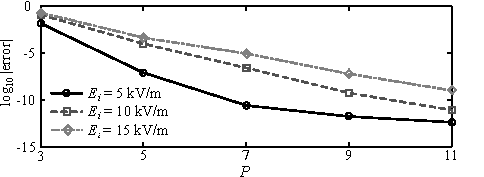
\includegraphics{convergence}
\caption{
Relative error of the spectrum at fundamental frequency for various $E_i$ values.}
\label{fig:convergence}
\end{figure}

\begin{figure}[!t]
\centering

\includegraphics{acceleration}
\caption{Acceleration spectrum obtained for an HBFE system of several harmonic
orders. The computations are made for $E_i = 15$~kV/m ($\gamma = 0.1$).}
\label{fig:acceleration}
\end{figure}

The efficiency of the DD technique can be assessed by its acceleration, that is
the ratio between time for a full domain computation and the corresponding DD 
computation (comprehensive of the Schur complement solution) \cite{Guarnieri2010}. 
Fig.~\ref{fig:acceleration} presents  the acceleration for each frequency point,
and for different values of $P$ at $E_i = 15$~kV/m. In general, higher order 
HBDDFE systems have lower acceleration, since the degrees of freedom dimensions
related to nonlinear media increase.
%With a $P=3$ system, the acceleration varies in the range [2.51,
%9.15], averaging to 4.18, and leading to an HBDDFE solution in 24\% of the
%time required by a full domain HBFE solution.

\section{Conclusion}
A harmonic balance approach to the DD-FE solution for the efficient analysis of 
waveguide devices containing nonlinear dielectrics has been 
presented and the accuracy of the multiharmonic solution 
discussed. 

\bibliographystyle{IEEEtran}
\bibliography{IEEEabrv,HBFEDD2}

\end{document}


